\documentclass[9pt,pdftex]{beamer}
\usepackage[latin1]{inputenc}
\usepackage[english]{babel}
%\usepackage{graphics}
\usepackage{graphicx}
\usepackage{hyperref}

\usepackage{units}
%\usepackage{listings}
%\lstset{%
%  language=C++,
%  numbers=left, 
%  numberstyle=\tiny,
%  frame=single
%}
%
\usepackage{amsmath}
\usepackage{amsfonts}
\usepackage{amssymb}

\usepackage{color}

\usepackage{amsmath}
\usepackage{tikz}
\usetikzlibrary{calc}
\usetikzlibrary{shapes}

\useoutertheme{infolines}
\usetheme[]{default}
\setbeamertemplate{navigation symbols}{}
\setbeamertemplate{bibliography item}[text]
\setbeamertemplate{blocks}[rounded][shadow=true]
\setbeamertemplate{caption}[numbered]
\definecolor{somegrey}{RGB}{240,240,240}

\setbeamercolor{block title}{bg=black!60!white,fg=white}
\setbeamercolor{block title alerted}{use=alerted text,fg=red,bg=black!60!white}
\setbeamercolor{block title example}{bg=black!20!white}

\hypersetup{
  colorlinks,
  linkcolor=blue!60!white,
  urlcolor=blue,
  urlbordercolor=blue%,% hyperlink borders will be red
%  pdfborderstyle={/S/U/W 1}% border style will be underline of width 1pt
}

%\addfootbox{bg=grey,fg=black}{\quad \insertshortauthor \hspace{.4\textwidth} \insertshortinstitute \hspace{.4\textwidth} \insertpagenumber}
\usepackage{listings}
\lstset{%
  language=C++,
  numbers=left, 
  numberstyle=\tiny,
  frame=single
}
%\renewcommand{\theenumi}{\alph{enumi}}
%\renewcommand{\labelenumi}{\theenumi)}
\begin{document}


% \pgfdeclareimage[height=1.5cm]{ATLASlogo}{img/AN_atlaslogo}
% \pgfdeclareimage[height=1.5cm]{FSPlogo}{img/FSPAtlas_logo}
 \pgfdeclareimage[height=.4cm]{license}{img/Full-CCBY3.0_88x31.png}
\titlegraphic{ \centering under CC  license \quad\pgfuseimage{license} \quad BY 3.0 }

\title[TBB]{ Pragmatic Introduction to Intel's Threading Building Blocks }
%\subtitle{- A  -}
\author[P. Steinbach]{Peter Steinbach}
\date{June 20th, 2012}

\institute[IKTP]{Institute for Nuclear and Particle Physics, TU Dresden}

\begin{frame}
  \begin{block}{Today's Question}
    \begin{center}
      How to implement parallel computing structures in C++?
    \end{center}
  \end{block}
  \vfill
  \begin{columns}[t]
    \begin{column}{.45\textwidth}
      \begin{block}{Serial Workflow}
        
\includegraphics[width=.9\textwidth]{img/Cream_puff_assembly_line}\cite{Wikicommons}
      \end{block}
    \end{column}
    \begin{column}{.45\textwidth}
      \begin{block}{Parallel  Workflow}
      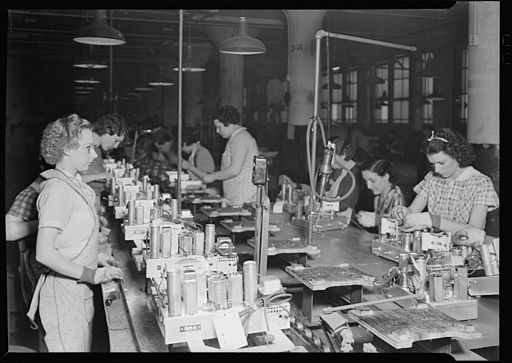
\includegraphics[width=.9\textwidth]{img/RadioAssembly}\cite{Wikicommons}
      \end{block}
    \end{column}
  \end{columns}
  \vfill
\end{frame}

\maketitle

\section[Intro]{Introduction}
\begin{frame}
\frametitle{A (bit of) Introduction}
\begin{block}{Let's assume ...}
  \begin{center}
    \begin{itemize}
    \item Your software \textbf{takes a too long} to complete.
    \item \textbf{You have identified a very CPU intense region in your code!} \\
    \item What to do? Let's go \textbf{parallel}.
    \end{itemize}
  \end{center}
\end{block}
\vfill
\begin{columns}[t]
  \begin{column}{.45\textwidth}
    \begin{block}{Multiple Processes}
      A \texttt{process}\cite{Wikipedia:Processes} is an instance of a computer program that is being executed. 
      It contains the program code and its current activity. A process is said to own the following resources: image of the executable machine code, memory (stack, heap), ...
    \end{block}
  \end{column}
\hfill
\pause
  \begin{column}{.45\textwidth}
    \begin{block}{Multiple Threads}
      A \texttt{thread}\cite{Wikipedia:Threads} of execution is the smallest unit of processing that can be scheduled by an operating system.
      A thread is a lightweight process. A thread is contained inside a process. 
      Multiple threads can exist within the same process and share resources (memory, ...).
    \end{block}
  \end{column}
\end{columns}
\vfill
\end{frame}

\begin{frame}
  \frametitle{Parallel $\neq$ Parallel}
  \begin{block}{Does the computer architecture play a role?}
    For Multi-Threading and Multi-Processing: No.\\
    For your problem: Yes!
  \end{block}
  
  \begin{columns}[t]
  \begin{column}{.45\textwidth}
    \begin{center}
      \emph{Shared Memory systems}\\[24pt]
    \end{center}
%    \includegraphics[width=.9\textwidth]{img/SimpleVonNeumann}\\[36pt]
    \includegraphics[width=.9\textwidth]{img/MultipleVonNeumann}\\
  \end{column}
\hfill
  \begin{column}{.45\textwidth}
    \begin{center}
      \emph{Shared/Distributed Memory systems}\\[24pt]
    \end{center}
    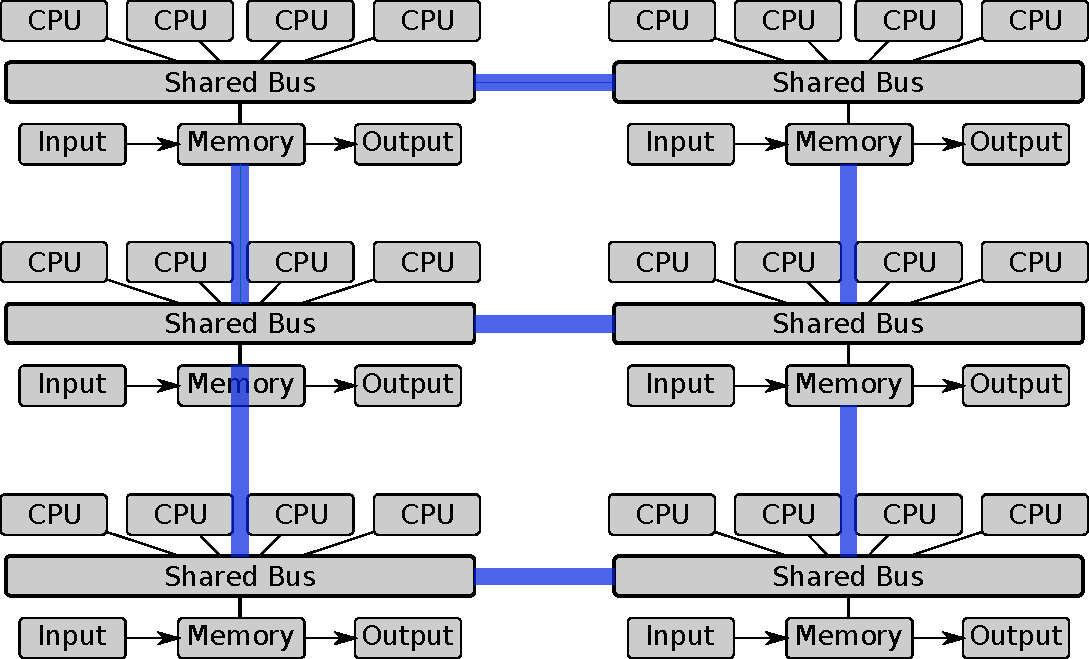
\includegraphics[width=.9\textwidth]{img/BatchVonNeumann} \\
      \end{column}
\end{columns}
\end{frame}


\begin{frame}
  \frametitle{Let's go for Multi-Threading}
  \begin{block}{I assume ...}
    \begin{itemize}
    \item your serial algorithm cannot be optimised further
    \item problem domain can be decomposed
    \item speed-up through multi-threading of code is high to justify
      coding effort
    \end{itemize}
  \end{block}
  \pause
  \begin{columns}
    \begin{column}{.45\textwidth}
      \begin{alertblock}{Always remember}
        Implementing concurrency (i.e. multi-threading) is quite an effort!\\
      \end{alertblock}
    \end{column}
    \begin{column}{.45\textwidth}
      \begin{center}
        
\includegraphics[width=.9\textwidth]{img/nebu_work}\cite{OpenClipart}
      \end{center}
    \end{column}
  \end{columns}

\end{frame}

\begin{frame}
  \frametitle{What library to pick?}
\begin{columns}
    \begin{column}{.45\textwidth}
      \begin{block}{Explicit Threading Libraries}
        Provides low level primitives (such as thread objects etc.)
        \begin{itemize}
        \item C++03 does support threads
          \begin{itemize}
          \item \href{http://www.boost.org/doc/libs/1_49_0/doc/html/thread.html}{Boost.Threads}
          \item \href{http://www.yolinux.com/TUTORIALS/LinuxTutorialPosixThreads.html}{POSIX threads}
          \end{itemize}
        \item C++11 does \texttt{std::thread}
        \end{itemize}
      \end{block}
    \end{column}
    \begin{column}{.45\textwidth}
      \begin{block}{Implicit Threading Libraries}
        Provide higher level API that encapsulate thread control
        \begin{itemize}
        \item \href{http://openmp.org/wp/}{OpenMP}
        \item \href{http://www.apple.com/osx/what-is/\#grandcentral}{Apple's Grand Central Dispatch}
        \item \href{http://threadingbuildingblocks.org/}{Intel Threading Building Blocks}
        \end{itemize}
      \end{block}
    \end{column}
  \end{columns}
\vfill
\begin{alertblock}{For me as a scientist ...}
  by first approximation, implicit libraries are my first choice (hide threading details, provide API for most common problems).
\end{alertblock}
\end{frame}

\section[TBB]{Intel Threading Building Blocks}
\begin{frame}
  \frametitle{Intel Threading Building Blocks}
  \begin{block}{Generalities}
    \begin{itemize}
    \item Open Source C++ library (\href{http://gcc.gnu.org/onlinedocs/libstdc++/manual/bk01pt01ch01s02.html}{GPLv2})
    \item sponsored by Intel\textsuperscript{\texttrademark}
    \item runs on shared memory x86 architectures
    \item runs with Windows, Mac and Linux (MS Visual++, icc, gcc, ... )
    \item current version: 4.0 
    \end{itemize}
  \end{block}

  \begin{block}{Design}
    \begin{itemize}
    \item generic template library
    \item design similar to STL (templated algorithms interfaced with templated container types)
    \item developer friendly (exceptions, compiler checks type safety)
    \item good documentation (\href{http://threadingbuildingblocks.org/documentation.php}{tutorials, Examples, Code reference} available online
    \item some low-level features: custom memory allocators, atomic operation identifiers ...
    \end{itemize}
  \end{block}
\end{frame}


\begin{frame}
  \frametitle{A Quick Look Inside}
  \begin{block}{Containers}
    \begin{itemize}
    \item \texttt{tbb::concurrent\_vector}
    \item \texttt{tbb::concurrent\_hash\_map}
    \item \texttt{tbb::concurrent\_queue}
    \end{itemize}
  \end{block}

  \begin{block}{Algorithms}
    \begin{itemize}
    \item \texttt{tbb::parallel\_do}
    \item \texttt{tbb::parallel\_for} (*)
    \item \texttt{tbb::parallel\_sort}
    \item \texttt{tbb::parallel\_reduce} (*)
    \item \texttt{tbb::parallel\_pipeline}
    \item ...
    \end{itemize}
  \end{block}
  
\end{frame}

\begin{frame}[fragile]
  \frametitle{Example 1: A simple logger}
  \begin{block}{Serial Version}
    \small
    \begin{lstlisting}[]
for(int i = 0;i<nIterations;i++){ 
  std::cout << "iteration "<< i << std::endl; 
}
    \end{lstlisting}
  \end{block}
\pause
   \vfill
   \begin{block}{Parallel}
     \small
     \begin{lstlisting}[]
//...  
int grainsize = nIterations/nThreads;
tbb::parallel_for(tbb::blocked_range<size_t>(0, 
                                             nIterations,
                                             grainsize), 
                  NumPrinter() 
                  ); 
//...
     \end{lstlisting}
   \end{block}

\end{frame}

\begin{frame}[fragile]
  \frametitle{Example 2: A throwing random numbers}
  
   \begin{block}{Parallel Reduce}
     \small
     \begin{lstlisting}[]
Sum sumWorker(data);
tbb::parallel_reduce(tbb::blocked_range<size_t>(0,
                                                nIterations,
                                                grainsize),
                     sumWorker);
     \end{lstlisting}
   \end{block}

   \begin{block}{Difference to Example 1}
     \begin{itemize}
     \item \texttt{Sum} has no const \texttt{operator()}
     \item \texttt{Sum} has dedicated constructor with \texttt{tbb::split} macro
     \end{itemize}
   \end{block}
\end{frame}

\begin{frame}
  \frametitle{Attention}
  \vfill
  \begin{center}
    \includegraphics[width=.6\textwidth]{img/Bundesarchiv_Bild_183-1984-0814-033_LPG_Neukirchen}\cite{Wikicommons}
    \begin{alertblock}{Always ...}
      \begin{center}
        Compare Parallel and Serial Performance!\\
        (was/is the effort worthwhile?)
      \end{center}
    \end{alertblock}
  \end{center}

  \vfill
\end{frame}

\begin{frame}
  \frametitle{Summary}
  \vfill
  \begin{block}{My Conclusion}
    \begin{itemize}
    \item Multi-threading is NO SILVER BULLET
    \item TBB is a well composed template library
    \item its open source (so sciencists can go for it)
    \item it offers high-level functionality that encapsulates low level thread management
    \item it offers an API to approach/solve most problems with parallel solutions
    \item it has a learning curve
    \end{itemize}
  \end{block}

  \vfill
  \begin{block}{further reading I recommend}
    \begin{itemize}
    \item \href{http://threadingbuildingblocks.org/documentation.php}{online} TBB documentations
    \item \href{http://www.dailymotion.com/playlist/x1pc0m_Intel_Academic_EMEA_intro-to-parallel-programming/1\#video=xksoje}{video lecture} series by Clay Breshears
    \end{itemize}
  \end{block}
\end{frame}

\section{References}
\scriptsize
\begin{frame}
  \frametitle{References}
  \bibliographystyle{plain} 
  \bibliography{June20.TBB}
\end{frame}

\section{Legal Disclaimer}
\begin{frame}
  \vfill
  \begin{block}{License}
    This talk is published under the creative commons BY licence 3.0. For details, see \href{http://creativecommons.org/licenses/}.\\
    All contained material was created by the author or obtained from creative common licensed sources (as indicated). For questions, concerns, criticism and improvements, contact: \href{mailto:Peter.Steinbach@tu-dresden.de}.
  \end{block}
  \vfill
\end{frame}

\end{document}




